%% ---------------------------------------------------------------
%% $URL: https://repository.cs.ru.is/svn/thesis-template/trunk/ruthesis/latex/DEGREE-NAME-YEAR.tex $
%% $Id: DEGREE-NAME-YEAR.tex 360 2019-02-13 22:04:35Z foley $
%% This is a template LaTeX file for dissertations, theses, or reports at Reykjavík University
%% 
%% Comments and questions can be sent to the RU LaTeX group (latex AT list.ru.is) 
%% ---------------------------------------------------------------

%% METHOD:
%% 0) Read ruthesis/thesis-instructions.pdf
%%    If it is missing, goto https://repository.cs.ru.is/svn/thesis-template/trunk/ruthesis/thesis-instructions.pdf
%% 0.2) Subscribe to the announcements email list at
%%    https://list.ru.is/mailman/listinfo/latex-announcements
%% 1 LaTeX instructions.tex or goto http://afs.rnd.ru.is/project/thesis-template/trunk/ruthesis/latex/instructions.pdf
%% 2) Copy the template files (or unzip) to your working area
%% 3) Rename this file (if needed) with your information e.g. MSC-FOLEY-2007.tex
%% 4) Modify this file to fit your needs (please follow all comments below in the text)
%% 5) For making bibliographies, run "biber".  You can also change
%%    this back to "bibtex".  See below in "Bibliography options".

%%%%%%% CHOOSE ONE OF THESE %%%%%%%%%%%%%%%
%% projectreport: Project report (CS)
%% bachelors: Bachelor of Science thesis
%% masters: Master of Science thesis
%% doctorate: Doctor of Philosophy dissertation
%
%%%%%%% CHOOSE ONE OF THESE %%%%%%
%% 
%% draft: speed up processing by skipping graphics and adding useful
%%     information for editing.  Also sets spacing to double so that it is easier to
%%     write editing marks on paper copy.
%% proof:  proofreading version (final formatting with warnings)
%% final: generate document for submission, removing FIXMEs, and
%%     other markup.  Throw error if any fatal FIXMEs still in document.
%%
%%%%%%% CHOOSE ONE OF THESE IF APPLICABLE %%%%%%
%%
%% deptsse: School of Science and Engineering
%% deptscs: School of Computer Science
%%
%%%%%%%% CHOOSE ANY COMBINATION OF THESE %%%%%%%%%%%%
%%
%% forcegraphics: force graphics, etc. to be included, even in draft mode
%% debug:  writes more messages to the log file, adds debugging output 
%%     and sizing boxes
%% icelandic: thesis is in Icelandic
%% oldstyle:  use the PhD headers and footers from the old CS template
%% online: for online versions (skip blank pages)
\documentclass[online,masters,deptscs,forcegraphics,draft]{ruthesis}

%%%%%%%%%%%%%%%%%%%% TeXStudio Magic Comments %%%%%%%%%%%%%%%%%%%%%
%% These comments that start with "!TeX" modify the way TeXStudio works
%% For details see http://texstudio.sourceforge.neit/manual/current/usermanual_en.html   Section 4.10
%%
%% What encoding is the file in?
% !TeX encoding = UTF-8
%% What language should it be spellchecked?
% !TeX spellcheck = en_US
%% What program should I compile this document with?
% !TeX program = xelatex

%%%%%%%%%%%%%%%%%%%% Bibliography options %%%%%%%%%%%%%%%%%%%%%
%% We suggest switching from bibtex to biblatex/biber because it is better able
%% to deal with Icelandic characters and other bibliography issues
%% As long as you use biblatex instead of bibtex by itself, it will at least
%%  generate a document without errors.
%% !!!If you are using TeXStudio, don't forget to update the bibliography setting!!!
\usepackage[backend=biber,bibencoding=utf8,style=ieee]{biblatex}
%\DeclareLanguageMapping{american}{american-apa}  
% need to declare mapping for style=apa to alphabetize properly
% If you set backend=bibtex, it will use bibtex for processing (old way)
%    this can work with Icelandic characters, but you may get weird results.
%    bibtex does not know how to sort Þ and ð
% if you set backend=biber, you can use UTF8 characters such as Þ and
%     ð  but you will have to remember to switch from using bibtex to 
%     biber in your client
% If you use JabRef, make sure the file is encoded in UTF-8 which is
%    not the default.

%% This tells TeXStudio to use biber
% !TeX TXS-program:bibliography = txs:///biber
%% This also sets the bibliography program for TeXShop and TeXWorks
% !BIB program = biber

% Where is your reference library?
\addbibresource{references.bib}
\addbibresource{more_references.bib}

%%%%%%%%%%%%%%%%%%% CUSTOMIZATIONS %%%%%%%%%%%%%%%%%%%%%%%%%%%%%
%% It is not recommended that you customize this file nor
%% ruthesis.cls.  Just fill in the necessary fields.  You should put
%% your macros and packages into a separate file so that it is easier
%% to use updates to the template.  The custom.sty file was created
%% for this reason.  We load this much later so that it can overrite
%% any existing settings
\IfFileExists{custom.sty}{\usepackage{custom}}{}


%%%%%%%%%%%%%%% INFORMATION %%%%%%%%%%%%%%%%%%5
%% University information must be multilingual to deal with the
%%  required cover pages and abstract on thesis
%% NOTE: This may not be required for other reports!!!

%% Babel Icelandic macros are setup  on RedHat at
%% /usr/share/texlive/texmf-dist/tex/generic/babel/icelandic.sty
%% /usr/share/texlive/texmf-dist/tex/generic/babel-icelandic/icelandic.ldf


%% Multilingual macros
%\newML{macroname}{englishword}{icelandicword}
%  creates \macronameML
%    \MLmacroname[english] - returns the english word
%    \MLmacroname[icelandic] - returns the icelandic word
%    \MLmacroname  - uses the current language setting
% Some useful ones have already been defined, but can be redefined
%% Predefined: \MLIceland \MLReykjavikUniversity \MLUniversityIceland

%% What institute?  Default is RU.
%\setInstitution{\MLReykjavikUniversity}
% \newML{InstitutionAddress}{Menntavegur 1\\101 Reykjavík, Iceland}
% {Menntavegi 1\\101 Reykjavík, Ísland}
% \setInstitutionAddress{\MLInstitutionAddress}
% \newML{Tel}{Tel.}{Sími}
% \setInstitutionPhone{\MLTel{} +354 599 6200\\
% Fax +354 599 6201}
% \setInstitutionURL{www.ru.is}


%% ONLY SET DEPARTMENT IF YOU HAVE NOT USED THE deptsse or deptscs OPTION!
%% Department and degree program
%\newML{ND}{New Department}{Nytt deild}
%\setSchool{\MLND}

%% Set your program of study
\newML{program}{Software Engineering}{hugbúnaðarverkfræði}
\program{\MLprogram}

%% Degree long name.  If not already defined, you can create a macro
%\newML{DEGREE}{English Degree Name}{Icelandic Degree Name}
%% Default is set based upon doctorate vs masters option
%% Predefined: \MLMSc \MLPhd
%\setDegreelong{\MLMSc}

%% Degree abb, change if default is not right
%% Default is set based upon doctorate vs masters option
%\degreeabbrv{Sc.D.} 

%\setFrontLogo{reyst-logo}
%% Use this if you need a different front logo on the first page
%% e.g. reyst-logo

%% Date in english and icelandic
%% NOTE: THIS IS THE DATE OF THE SUPERVISOR'S SIGNATURE!!!!!!
%% Predefined: \MLjan, \MLfeb, \MLmar, ... \MLdec
%\whensigned{day}{month}{year} %day is only used on some formats, but you must put something.
\whensigned{10}{\MLapr}{2022}

%% Title first in English then Icelandic
%% You need to put both a normal case and ALL CAPS version into the macros.
%%
\newML{Title}{Forecasting Solar Power Production Using Deep Learning and High Resolution Weather Forecasts}{Sólarorkuframleiðsluspár með djúpnámi út frá háupplausnar veðurspám}
\newML{TITLE}{FORECASTING SOLAR POWER PRODUCTION USING DEEP LEARNING AND HIGH RESOLUTION WEATHER FORECASTS}{SÓLARORKUFRAMLEIÐSLUSPÁR MEÐ DJÚPNÁMI ÚT FRÁ HÁUPPLAUSNAR VEÐURSPÁM}
%%
\setTitle{\MLTitle}{\MLTITLE}
%% ***** Special Titles ******
%% If the title must be formatted specifically for the cover page or internal pages
%% (typically via line-breaks using the \newline command) then the following commands must be used 
%%
%\setTitleCover{\MLTITLE}
%% These two for the internal cover pages, usually not needed
%\newML{TitleInternal}{Internal Title}{Icelandic Internal Title}
%\setTitleInternal{\MLTitleInternal}

%% Author name (should be the same in any language, if not use \newML)
%% If you are writing a Project report with multiple authors, separate them with \\:
%% To keep the names typeset together, you want to use non-breaking spaces: ~
%\author{Firstname1~Lastname1\\Firstname2~Lastname2}
\author{Einar~Helgi~Guðmundsson}

%% If the name must be formatted specifically for the signature page
%% (typically via line-breaks) then the following command must be used 
%\setAuthorSignature{Student\\Name}
%% This macro adjusts the author name in the headers of the oldstyle formatting
%\setAuthorHeader{StudentLast}

%%% TODO:  Move the bachelor's form separately -- it confuses people. --foley
%%%%%%%%%%%%%%%%%%%%%%%%%% Project Report or Bachelor's Only!!! %%%%%%%%%%%%%%%%%%%%%%%%%%%%%%%%%%%%%%%%%%%
\setCourse{VT LOK 1012}

%%%%%%%%%%%%%%%%%%%%%%%%%% Bachelors Only!!! %%%%%%%%%%%%%%%%%%%%%%%%%%%%%%%%%%%%%%%%%%%
\setID{160992--2989}%kennitala
\setSemester{2022-2}
\setShortSignedDate{10.4.2022}

\setOrganization{Belgingur ehf.\\Grensásvegur 9\\108 Reykjavík}
\setSubProgram{Hugbúnaðarverkfræði}

%% If the thesis is confidential, uncomment this with the date it can be released
%\setClosedDistribution{10.1.2016}%

%% Put your keywords here in English, then Icelandic.  Separate them with commas.
\newML{keywords}{Deep Learning, Solar Power, Forecast}{Djúpnám, Sólarorka, spá}
\setKeywords{\MLkeywords}

%%%%%%%%%%%%%%%%%%%%%%%%%%% Masters Only!! %%%%%%%%%%%%%%%%%%%%%%%%%%%%%%%%%%%%%%%%%%%%
%% How many credits (ECTS) on Master's degree
%% Usually 30 or 60
\ects{60}

%%%%%%%%%%%%%%%%%%%%%%%%%%% Doctorate Only!! %%%%%%%%%%%%%%%%%%%%%%%%%%%%%%%%%%%%%%%%%%
%% Some Computer Science Thesis have an ISSN number.
%% Most other documents do not.
%\bookidnumber{ISSN: 1670-8539} 
%% ID numbers are optional, but nice for sorting in libraries

%% International Standard Book Number (ISBN)
%% This is what most people should use if the thesis is being published.

%% International Standard Serial Number (ISSN)
%% This is usually only for a PhD dissertation as part of a series when published
%%   Computer Science: 1670-8539 

%% Additional degrees?  (optional, usually not needed)
%\adddegree{(list of degrees in appendix)}{(sjá lista yfir prófgraður í viðauka)}
%%%%%%%%%%%%%%%%%%%%%%%%%%%%%%%%%%%%%%%%%%%%%%%%%%%%%%%%%%%%%%%%%%%%%%%%%%%%%%%%%%%%%%%%


%% List the entire committee.  Each member has a name (degree should be omitted, unless it is not PhD),
%% Supervisor(s) must appear first
%% On a Bachelors, there is usually only one supervisor and one examiner.

%% Format for each entry:
%%  \personinfo{Name}{Role}{Job Title}{Company/institution}{Country}
%% Predefined macros: \MLSupervisor \MLSupervisors \MLExaminer \MLExaminers

%% Change these to singular/plural as needed.
%% Just uncomment and change the plurality of the macro.
%\setSupervisorHeading{\MLSupervisors}
%\setExaminerHeading{\MLExaminer}

%% Predefined macros:
%% \MLSeniorProfessor \MLProfessor \MLAssociateProfessor \MLAdjunctProfessor \MLEmeritusProfessor \Iceland
%% \MLReykjavikUniversity \MLUniversityIceland

%% Bachelors: primary advisor (Umsjónarkennari), ONLY ONE!
%% All others: As many as you want
\supervisors{
  \personinfo{Yngvi Björnsson}{\MLSupervisor}{\MLProfessor}{\MLReykjavikUniversity}{\MLIceland}
  \personinfo{Ólafur Rögnvaldsson}{Co-advisor}{Managing Director}{Belgingur ehf.}{\MLIceland}
%  \personinfo{Ian M. Great}{Co-advisor}{\MLProfessor}{Hochschule Düsseldorf}{Germany}
}

%% Bachelors: secondary advisor (Leiðbeinandi), ONLY ONE
%% All others: As many as you want
\examiners{
  \personinfo{Tough E. Questions}{\MLExaminer}{Associate Professor}{Massachusetts Institute of Technology}{USA}

}

%% An abstract is required to be in both Icelandic and English for most degrees.
%% It is considered good form to limit the abstract to a single paragraph in each language,
%%   at 300 words.  Refer to your degree's instructions.
%% Note: Icelandic quotation marks cannot be typeset using "` and "'.  You should use \enquote{}
%% this is probably due to interactions with the MultiLingual macros.
%% TODO: turn this into more sensible macros to avoid confusion --foley
\newML{AbstractText}{\lipsum[1]}  
% ipsum generaes text text
{\lipsum[1]} % Icelandic abstract goes here
\setAbstract{\MLAbstractText}


%%%%%%%%%%%%%%INDEX SETUP %%%%%%%%%%%%%%%%%%%%%%%%%%%%%%%%%%%%%%%%%%%%%%%%%%%%
%% Indexes, and other auto-generated material
%% The Memoir package (which we use) automatically generates the index
%% See section 17.2 on page 302 of the guide
%% http://texdoc.net/texmf-dist/doc/latex/memoir/memman.pdf
%% This means you have to run "makeindex DEGREE-NAME-YEAR"
%% !!!Do not load any of the index packages, they cause problems with Memoir!!!
%% !!!You have been warned!!!
%% Note that memoir changes the [] options to only be for filenames, not other options!
\makeindex{}
\indexintoc{}

%% For abbreviations, you may want to try
%% Watch out though, each new index writes another external file and 
%% latex can only write a limited number of them
%%\usepackage[intoc]{nomencl} % intoc: In Table of Contents
%% remember to run:
%% makeindex filename.nlo  -s nomencl.ist -o filename.nls

\finalifforcegraphics{hyperref} %hyperlinks even in draft mode
\usepackage[hidelinks]{hyperref} 
%% !!!Must be the last package loaded except otherwise mentioned!!!!
%% \usepackage{hypcap}  %% puts link at top of figure, must be after hyperref

%%%%%%%%%%%%%%%%%%%%%%%%%%%%%%%%%%%%%%%%%%%%%%%%%%%%%%%%%%%%%%%%%%%%%%%%%%
%%%%%%%%%%%%%%%%%%%%%%% DOCUMENT START %%%%%%%%%%%%%%%%%%%%%%%%%%%%%%%%%%%
\begin{document}
%% Some elements have different names on the RU Masters rules
%% They will be annotated with RUM: "name"
\frontmatter{} % setup formatting at beginning

%\frontcover{}%%If you want to see what it looks like with the printed cover
%% TODO:  link to fill-in PDF file on RU website

\frontrequiredpages{}%% the various signaturepages and abstract
%%% WARNING:  if you get an error on the previous line, it is probably because
%%% you put a bad macro or something strange in a title, author, or abstract.

\ifdraft{\coverchapter{Important!!!  Read the Instructions!!!} If you
  have not already done so, \LaTeX{} the \path{instructions.tex} to
  learn how to setup your document and use some of the features.  You
  can see a (somewhat recent) rendered PDF of the instructions included in this folder at \path{instructions-publish.pdf}.
  There is also more information on working with \LaTeX{} at
  \url{http://samvinna.ru.is/project/htgaru/how-to-get-around-projects-publish.pdf}.
  This includes common problems and fixes.

  This page will disappear in anything other than draft mode.}{}



%% Dedication is optional, comment out if it is absent
%% RUM: Not mentioned
\begin{dedications}
  I dedicate this to my spouse/child/pet/power animal.
\end{dedications}

\enableindents{}% turn on/off paragraph indents
% RUM: "Acknowledgements (optional)"
\coverchapter{Acknowledgements} 
\begin{quotation}
So long, and thanks for all the fish.
\end{quotation}\sourceatright{Douglas Adams\cite{adams84fish}}
\vspace{\baselineskip}

\draftnote{Acknowledgements are optional; comment this chapter out if they are absent
  Note that it is important to acknowledge any funding that helped in the work}

This work was funded by \the\year~RANNIS grant ``Survey of man-eating Minke whales'' 1415550.
Additional equipment was generously donated by the Icelandic Tourism Board.

\coverchapter{Preface}
% RUM: "Preface (optional)"
This dissertation is original work by the author, Einar~Helgi~Guðmundsson.
Portions of the introductory text are used with permission from
Student et al.\cite{student2015awesome} of which I am an author.

  
\draftnote{The preface is an optional element
  explaining a little who performed what work.  See
  \url{https://www.grad.ubc.ca/sites/default/files/materials/thesis_sample_prefaces.pdf}
  for suggestions.
  
  List of publications as part of the preface is
  optional unless elements of the work have already been published.
  It should be a comprehensive list of all publications in which
  material in the thesis has appeared, preferably with references to
  sections as appropriate.  This is also a good place to state
  contribution of student and contribution of others to the work
  represented in the thesis.}

%\coverchapter{Publications}
%% RUM: Not mentioned, this was found in the CS thesis template.  
%% Maybe more applicable to PhD dissertations?
%%% Probably a duplication from before Preface became standard.

\starttables{}% setup formatting
%% TOC, list of figures and list of tables are required
\tableofcontents{}\clearpage%%RUM: "Table of contents"
\listoffigures{}\clearpage%%RUM: "List of figures"
\listoftables{}\clearpage%%RUM: "List of tables"

%\coverchapter{List of drawings and enclosed material}
%RUM: "List of drawings and enclosed material, e.g. CD(as appropriate)"

\listoffixmes{}
% if using fixme package, lists what needs to be done

%% The list of abbreviations is an example of a special list
%% Other lists may be added, such as lists of algorithms, symbols, theorems, etc.
%% IN CS PhD, this is sometimes centered.
\coverchapter{List of Abbreviations}%%RUM: Not mentioned
\begin{tabular}{ll}
MSc &Masters of Science\\
PhD &Doctor of Philosophy\\
\end{tabular}

\coverchapter{List of Symbols}%%RUM: Not mentioned
\begin{tabular}{lll}
Symbol &Description &Value/Units\\
$E$ &Energy &\si{\joule}\\
$m$ &Mass &\si{gram}\\
$c$ &Speed of Light &\SI{2.99E8}{\meter\per\second\square}\\
\end{tabular}

%% This command prepares for the actual text, e.g. by 
%% calling \mainmatter{}
\starttext{}

%% ---------------------------------------------------------------
%% From this point on, it is standard Latex, except the very end.
%% This is a "report"-based template, so the top-level heading 
%% is \chapter{}

%% WARNING: Make sure that all of these files (and any new ones)
%% are UTF-8 otherwise you will get weird encoding errors.

%% The default division is IMRAD, you may want to divide differently
%% See the introduction for guidance.

\chapter{Introduction\label{cha:introduction}}

Solar power production is extremely dependent on weather conditions \cite{lin_temporal_2020, lee_forecasting_2018, jaidee_very_2019, su_machine_2019, jang_solar_2016}. A single cloud can seriously impact the production of a solar farm. Such unreliability in a power production system is highly undesirable, since production must match demand \cite{lee_forecasting_2018}. When solar power production falls, the power demand it was serving must be fulfilled by other means. Fossil fueled power plants are generally kept on standby, waiting to fulfill this demand \cite{lee_forecasting_2018}. These plants often take hours to start, generally pollute more than other plants and are very expensive to run \cite{lee_forecasting_2018}.
Reliable and accurate forecasts of the fluctuations in solar power production can give power grid operators notice and insight into future power production \cite{lee_forecasting_2018}. This notice enables planning for the dips in power production and making arrangements into the future. This provides the tools to reduce the cost and pollution of power generation as well as increasing the reliability of power delivery to consumers \cite{lee_forecasting_2018}.
Recent advancements in deep learning have unlocked new tools that have been shown to be extremely effective in predicting the future behavior of a system given enough relevant data.\\

%% \ifdraft only shows the text in the first argument if you are in draft mode.
%% These directions will disappear in other modes.
\ifdraft{State the objectives of the exercise. Ask yourself:
  \underline{Why} did I design/create the item? What did I aim to
  achieve? What is the problem I am trying to solve?  How is my
  solution interesting or novel?}{}

\section{Background}

Recurrent Neural Networks (RNNs), especially Gated Recurrent Units (GRUs) and Long-Short Term Memory (LSTM) cells \cite{Goodfellow-et-al-2016} along with more advanced derivatives have been shown to be able to achieve good results when trained on previous weather and power generation data \cite{lin_temporal_2020, lee_forecasting_2018, jaidee_very_2019, su_machine_2019}.
RNNs are a class of deep neural networks where nodes are connected in a temporal sequence, allowing the network to learn time based data efficiently. LSTMs and GRUs are types of RNNs in which, the nodes in the network have additional stored states controlled by the network via mechanisms that use time delays or feedback loops \cite{Goodfellow-et-al-2016, noauthor_recurrent_2021}.\\
Lin et al. \cite{lin_temporal_2020} showed that while the more traditional GRUs and LSTMs show good performance on the task, Temporal Convolutional Neural Networks (TCNN) can show even better performance. \textit{"TCNN is a novel convolutional architecture designed for sequential modelling, which combines causal and dilated convolutions
and residual connections"} \cite{lin_temporal_2020}. \\
Jaidee et al. \cite{jaidee_very_2019} showed that for very short term predictions, on the time scale of a few hours, LSTMs, GRUs and derivative methods show relatively similar performance. This timescale is where it is critical to accurately predict cloud movements. 
These methods have been taken as far as building genetic algorithms to generate the optimal neural network for the purpose \cite{jaidee_very_2019}. These genetic algorithms operate on the same principals as animal breeding. They generate multiple candidate neural networks and use the best networks as a base to generate new networks for the next generation. This is done for multiple generations and in the end the best neural network generated is used \cite{jaidee_very_2019}.\\
Su et al. \cite{su_machine_2019} did extensive experimentation on more conventional neural networks and newer, less known networks including  Non-linear Auto Regressive Neural Network (NARXNN), as well as various statistical approaches. When predicting power output, NARXNN takes in the current power output values and considers them as well as the past values of the power output of the system. These experiments showed that NARXNN had the best performance of these, by a rather large margin, and a hybrid method, of the better performing methods, showed even better results \cite{anderson_using_2018}. The statistical methods generally performed significantly worse in predicting the power output. \\
Satellite imagery has been used for predicting solar power output as well. A neural network was trained to predict solar power production, primarily from cloud cover information it learned from these satellite images \cite{jang_solar_2016}.\\



\ifdraft{Provide background about the subject matter (e.g. How was morse code
developed?  How is it used today?). 
This is a place where there are usually many citations.
It is suspicious when there is not.
Include the purpose of the different equipment and your design intent. 
Include references to relevant scientific/technical work and books.
What other examples of similar designs exist?
How is your approach distinctive?

If you have specifications or related standards, these must be
described and cited also.  As an example, you might cite the specific
RoboSub competition website (and documents) if working on the lighting system for an AUV\cite{guls2016auvlight}


\section{Transformers}
Hard to train
sequential
 -> parallelization hard
encoder/decoder instead. Attention. 
 Explain enc/dec
 Autoencoders generate same output as the input, so no labeled data is needed -> completely unsupervisd learning.
 Locality a problem with CNNs and RNNs. Can easily find local context but keeping on to context far apart in input is difficult. Enter transformers.
 Encoder reads blocks of data and uses that and previously generated data as inputs into decoder which generatesdata one point at a time.
 Attention. How you relate things to each other. i.e. input to output
 self attention. How do features in the input data relate to each other


\subsection{Encoder/decoder}

\subsection{Attention}
 
 
\section{Goals}

%% Glossary is broken, do not use --foley
% \gls{auv}\footnote{Autonomous Undersea Vehicle}.

% Notice that there is now information on the AUV in the Index and Acronyms.
% It isn't in the \gls{glossary} because we didn't put it there.
\index{AUV}
}{}


%%RUM: Introduction
\chapter{Methods}

In this chapter, we discuss our solution to the problem of predicting solar power production. We cover the data we had access to and ultimately selected to train the neural network with, and how we processed and structured the data. We explain the Temporal Fusion Transformer architecture and how we set it up and use it to achieve our goals.

\section{Data}
This work relies on two types of data, \emph{the ground truth}, the measured irradiance at the power station and \emph{the input}, the irradiance values from high-resolution weather forecasts for the area. The data spans the 425 days from August 1st 2020 to September 30th 2021 for the Ituverava solar power station run by Enel S.p.A. in Bahia, Brazil.

\subsection{Irradiance measurements}
Under certain circumstances irradiance values simulated after the fact can be accurate, however, this does not apply in all conditions, and real measured values are much more reliable \cite{gueymard_global_2008}. The irradiance was measured with seven Kipp \& Zonen CM21 pyranometers placed around the power station. The pyranometers have a reported maximum measurement error of 3\%. For input into the network, the highest and lowest measured values are dropped and the average value of the other five measurements is used. This data is provided with five-minute intervals, but the neural network operates hourly. To downsample the measurement data to an hourly format, we averaged the values for the twenty minutes before and after the beginning of each hour. Finally, the irradiance values were normalized linearly to the range $0.0-1.0$ before being input into the neural network.


\subsection{Forecast data\label{cha:forecast_data}}
The weather forecast data is provided by Belgingur ehf., Reykjavík, Iceland. We use irradiance values from historical 24-hour weather forecasts generated by their WRF model, discussed in Section~\ref{cha:WRF}. The forecasts have a temporal resolution of one hour and a spatial resolution of 2.5km. One of our models uses forecast data from a 3x3 grid centred on the solar power station, and the other model the data from only the centre of the grid. We use two irradiance values from the forecast, the downward irradiance and the downward diffuse irradiance. These irradiance values were also normalized linearly to the range $0.0-1.0$ before being input into the neural network.


\subsection{Error metric}
In other work done in this area, multiple error metrics are used. One error metric is used more commonly than others, Mean Absolute Percentage Error (MAPE) \cite{lin_temporal_2020, lee_forecasting_2018, jaidee_very_2019, su_machine_2019}, which is the reason that metric was chosen.
When working with near-zero values MAPE becomes unhelpful as it is calculated by dividing by that near-zero value, so all cases where the irradiance is less than 15\% of the maximum value in the data set are dropped. Hence we do not evaluate early morning or late evening performance.
While a valuable metric, MAPE does not  fully represent the function of the model. Other factors like confidence, discussed in Section~\ref{sec:loss_function} and deviance from total irradiance for the day also represent key factors in the usefulness of the model.




\section{Tools}
The neural network was implemented in PyTorch 1.11 and PyTorch Forecasting 0.9.0. We used an NVIDIA GeForce RTX 3080Ti graphics card using CUDA for training. The computer had an AMD Ryzen 9 5950X CPU, 32GB of RAM and was running Windows 11.
This allowed for quick training of models, as with the relatively small amount of data, training a model took 5-10 minutes.

\newpage

\section{Model}
    \subsection{Temporal Fusion Transformer}
    
    \noindent We utilize a Temporal Fusion Transformer (TFT) model for the irradiance prediction.
    TFTs are  general networks which use attention at their core to generate multi-horizon forecasts with the ability to consider
    known information about the future, other related time series, and static metadata for the forecast \cite{lim_temporal_2020}. Figure~\ref{fig:tft_overviwew} shows an overview of how TFTs operate.
    
    \afterpage{%
    \begin{figure}
        \centering
         \makebox[\textwidth][c]{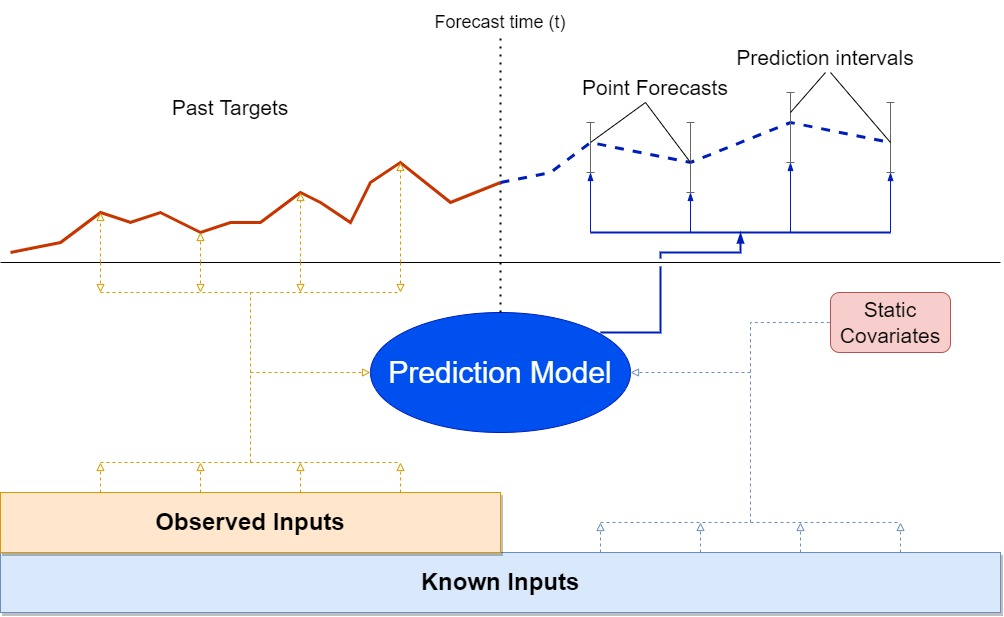
\includegraphics[scale=0.5]{imgs/TFT_overview.jpg}}
        \caption{An overview of the Temporal Fusion Transformer \cite{lim_temporal_2020}.
        \label{fig:tft_overviwew}}
    \end{figure}
    \clearpage
    }
    
    \noindent TFTs are composed of various components, each primarily addressing a single input type (i.e. static, known or observed inputs), aimed at maximizing the model versatility across various problems.
    

    
    \noindent\textbf{Gating mechanisms} identify and skip unused input data, granting models greater ability to work with less curated input data or datasets where it is unknown which parts are of significance.
    
    The Gated Residual Network (GRN) structure, shown in Figure~\ref{fig:ttgt_detail}, is a base building block of TFTs \cite{lim_temporal_2020}. It provides the model with the flexibility to choose the complexity of its input, more complex where needed, and less complex where not.
    

    
    \noindent\textbf{Variable selection networks} emphasize the most relevant inputs for every time step \cite{lim_temporal_2020}. Some variables may be more important than others, \enquote{TFT is designed to provide instance-wise variable selection through the use of variable selection networks applied to both static covariates and time-dependent covariates.} \cite{lim_temporal_2020} The variable selection mechanism also allows the model to remove noisy inputs that might have a negative effect on performance. \\
    \textbf{Static covariate encoders} encode static features into context vectors, integrating them into the network \cite{lim_temporal_2020}.  \\
    \textbf{Temporal processing} using a more traditional RNN sequence-to-sequence layer (see Section~\ref{cha:RNN}) for short term, local processing and the more novel multi-headed attention layer (see Section~\ref{cha:transformer}) for long term pattern capture \cite{lim_temporal_2020}.\\
    \textbf{Prediction intervals} in the form of quantile forecasts, discussed in Section~\ref{sec:loss_function}, display a confidence interval for the predictions \cite{lim_temporal_2020}. \\
    Figure~\ref{fig:ttgt_detail} shows a detailed view of the TFT structure as discussed. 
    
    \afterpage{%
    \begin{figure}
        \centering
         \makebox[\textwidth][c]{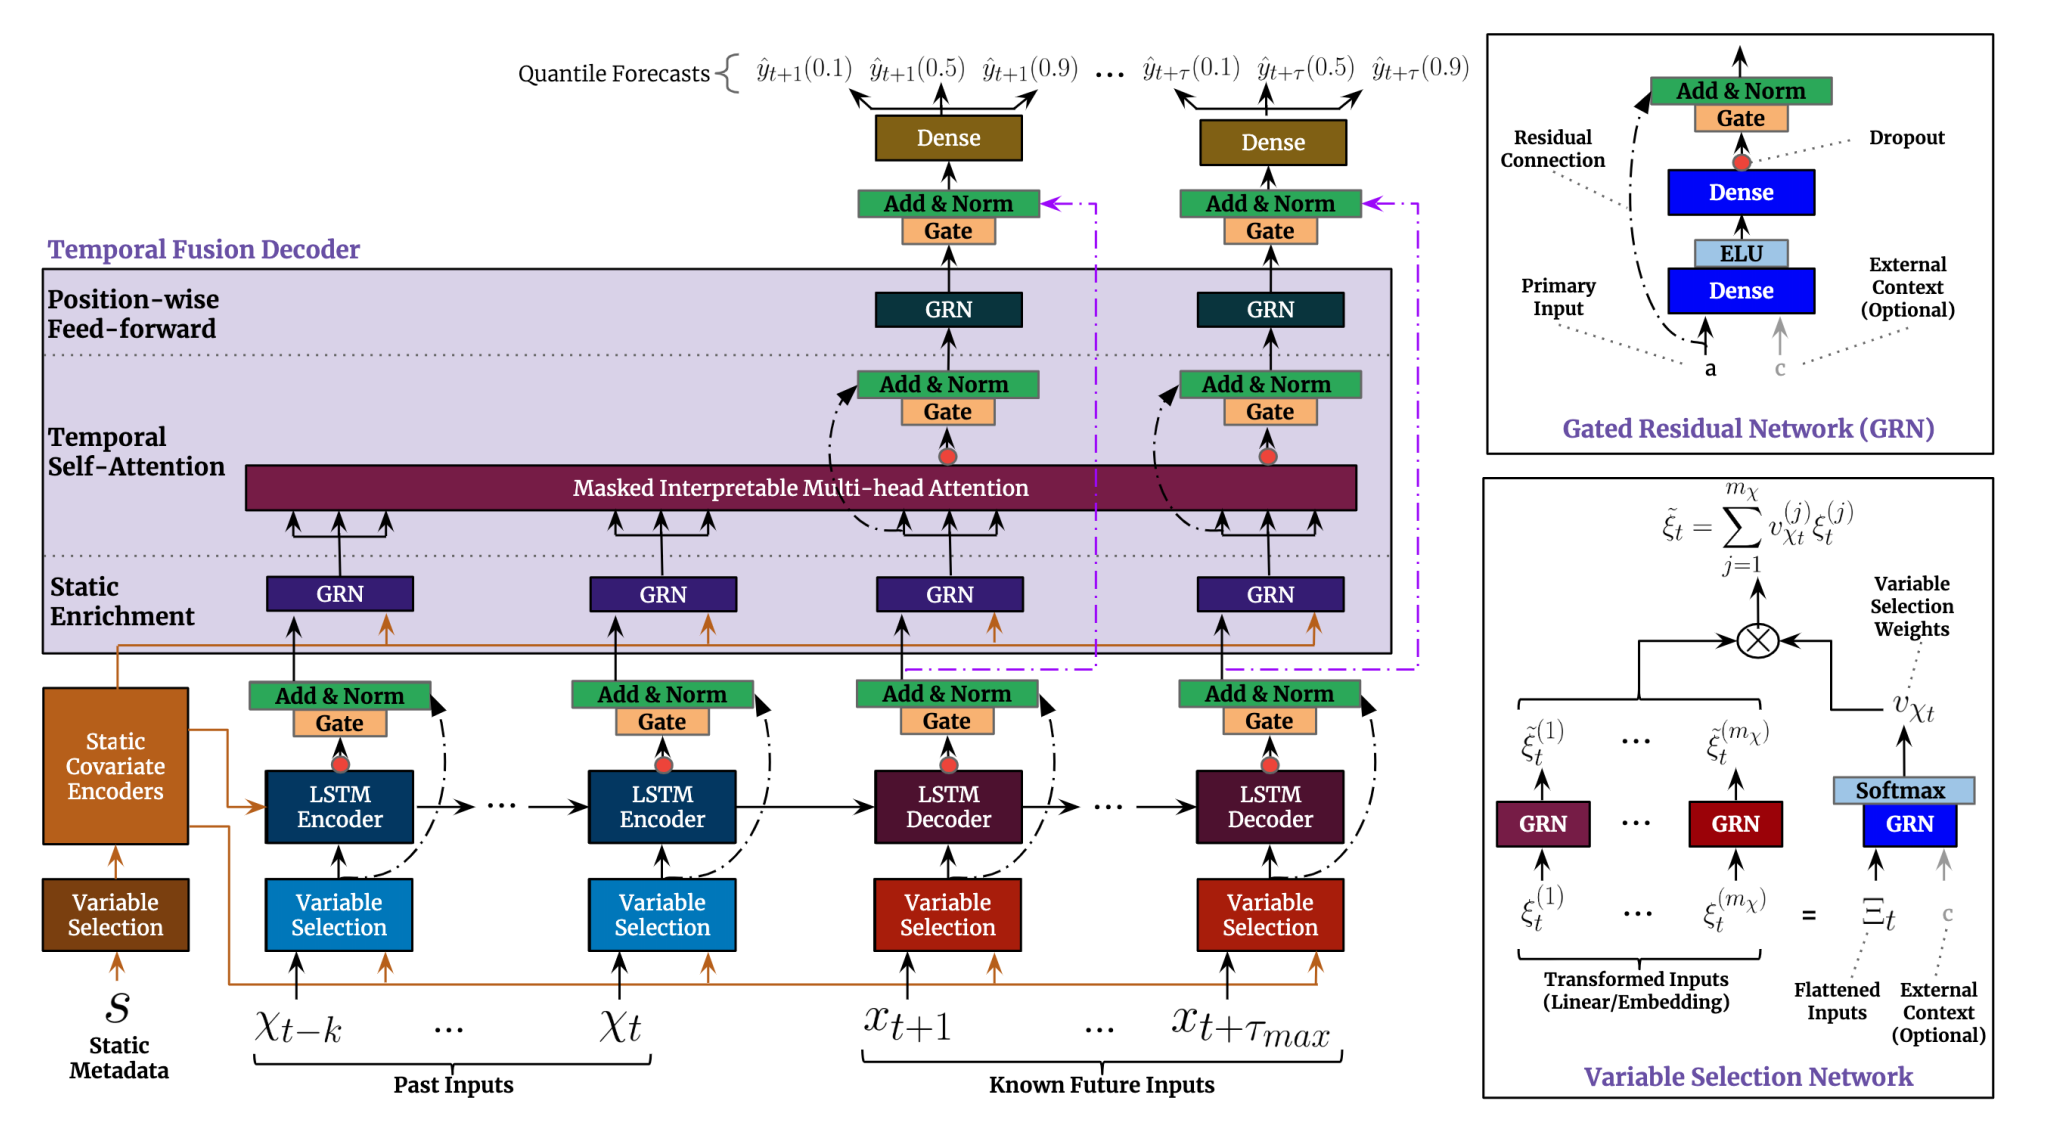
\includegraphics[scale=0.3]{imgs/TFT.png}}
        \caption{A detailed view of the architecture of the Temporal Fusion transformer \cite{lim_temporal_2020}.
        \label{fig:ttgt_detail}}
    \end{figure}
    \clearpage
    }

    \subsection{Setup}
    We trained two models. One which utilizes weather forecast data from an area surrounding the power station, and one which does not, as discussed in Section~\ref{cha:forecast_data}. The limited model is intended to show that the full model is able to glean additional information from the surrounding area data.
    
    
    \afterpage{%
    \begin{figure}
        \centering
        \makebox[\textwidth][c]{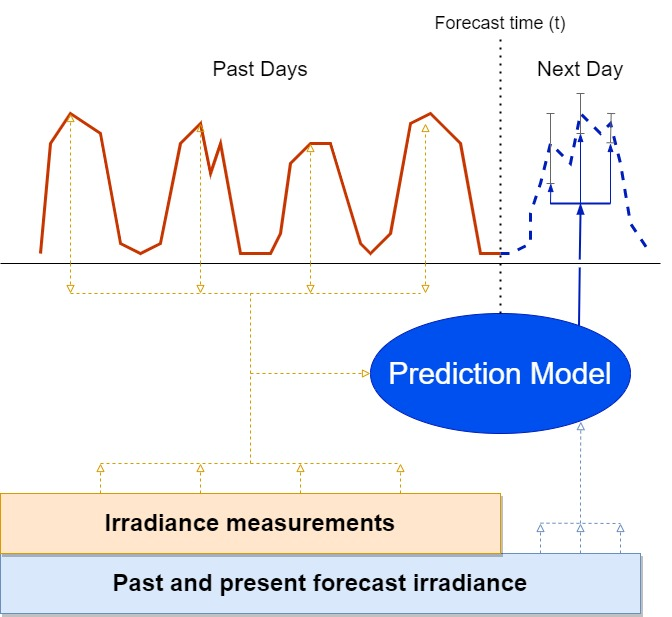
\includegraphics[scale=0.5]{imgs/solar_TFT_overview.jpg}}
        \caption{An overview of the setup of the neural network.
        \label{fig:solar_tft_overviwew}}
    \end{figure}
    \clearpage
    }


    \subsubsection{Inputs}
        The dataset was split into a training set, composing 70\% of the data, a validation set, composing 10\% of the data and finally, 20\% of the data was reserved for testing.
        Figure~\ref{fig:solar_tft_overviwew} shows how the observed inputs, the irradiance measurements, along with corresponding data from historical irradiance forecasts are used as training inputs.
        
    \pagebreak
    \subsubsection{Tuning}
        Significant tuning was done to optimize the performance of both models. Since the goal of tuning was not only to minimize Mean Absolute Percentage Error but balance that with the ability to recognize uncertainty, the process was very manual. Tables~\ref{tab:full_params} and \ref{tab:lim_params} show the selected hyperparameters for the full and limited models respectively.
        
        To avoid overfitting and to speed up the training of models, we used early stopping to stop training when the loss function optimization plateaued. 
        
        \vspace{1.5cm}
    
        \begin{table}[ht!]
        \begin{center}
        \caption{The full model hyperparameters.
        \label{tab:full_params}}
        \vspace{0.5cm}
        \begin{tabular}{|l|r|}
        \hline
        \textbf{Hyperparameter} & \textbf{Value} \\ \hline
        Learning rate            & 0.01         \\ \hline
        Batch size              & 24            \\ \hline
        Dropout                 & 0.1            \\ \hline
        Gradient clip           & 0.1           \\ \hline
        Hidden layer size            & 64         \\ \hline
        Hidden continuous size & 8         \\ \hline
        Attention head size   & 1         \\ \hline
        \end{tabular}
        
        \end{center}
        \end{table}
        
        \begin{table}[ht!]
        \begin{center}
        \caption{The limited model hyperparameters.
        \label{tab:lim_params}}
        \vspace{0.5cm}
        \begin{tabular}{|l|r|}
        \hline
        \textbf{Hyperparameter} & \textbf{Value} \\ \hline
        Learning rate            & 0.005         \\ \hline
        Batch size              & 24            \\ \hline
        Dropout                 & 0.1            \\ \hline
        Gradient clip           & 0.1           \\ \hline
        Hidden layer size            & 40         \\ \hline
        Hidden continuous size & 6         \\ \hline
        Attention head size    & 1         \\ \hline
        \end{tabular}
        
        \end{center}
        \end{table}
    
    \pagebreak
    \subsubsection{Loss function}\label{sec:loss_function}
    The loss function used for Temporal Fusion Transformers is quantile loss, as it is an integral part of generating the confidence intervals of the model \cite{lim_temporal_2020}.
    A model's prediction is a random value within a probability distribution \cite{wen_multi-horizon_2018}. If we make multiple predictions we can estimate this probability distribution by seeing within what range a selected proportion of the predictions fall \cite{koenker_quantile_2001}. PyTorch Forecasting's quantile loss function takes the Mean Absolute Error (MAE) of three quantiles, 90\%, 50\% and 10\%. This gives a good picture of the model's confidence in a prediction. A smaller quantile range indicates more confidence. 
    
    
    %%RUM: "Methods"
\chapter{Results}

In this section you discuss any issues that came up while developing
the system.  If you found something particularly interesting,
difficult, or an important learning experience, put it here.  This is
also a good place to put additional figures and data.

\lipsum[28-34]

%%% Local Variables: 
%%% mode: latex
%%% TeX-master: "DEGREE-NAME-YEAR"
%%% End: 
%%RUM: "Results"
\chapter{Discussion}
%In this section you discuss any issues that came up while developing
%the system.  If you found something particularly interesting,
%difficult, or an important learning experience, put it here.  This is
%also a good place to put additional figures and data.
Mean Absolute Percentage Error (MAPE) does not tell the whole story of a model's performance. The true measure of performance is how useful the model output is to energy producers. The model's confidence in a prediction is almost as important as the accuracy of the prediction and the total energy produced over the day matters.
The forecast downward shortwave irradiance, the largest factor in measured irradiance, rarely drops. It is almost exclusively on very high variance days that it deviates from a sine wave. The downward diffuse shortwave irradiance, the other network input data value, is a much smaller part of the total irradiance and has, to the bare eye, seemingly no correlation with the observation values. Despite this, the models show generally fantastic performance in predicting the irradiance.
The full model was able to utilize the forecast data from the surrounding area to achieve noticeably better performance. Of course, since the limited model uses only one ninth the data of the full model, some hyperparameter tuning had to be done to optimize its performance and some of the performance difference could be explained by worse optimization.
With the data at hand, it is not possible to separate the performance of the weather forecast model producing our input data and the performance of our models. We do not know how close this model comes to maximizing the information available in the input data.

Fig.~\ref{fig:disc_low} shows side-by-side the two models' performance for the same calm day. The full model was able to track the observations more closely with more confidence. This was typical for all calm days.
\begin{figure}[ht!]
    \centering
    \subfloat[Full model]{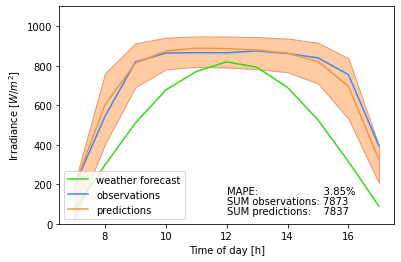
\includegraphics[scale=0.5]{imgs/graphs/disc/disc_med_full.png}}\qquad
    \subfloat[Limited model]{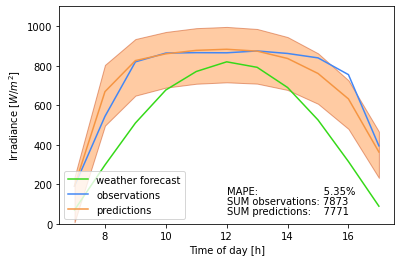
\includegraphics[scale=0.5]{imgs/graphs/less/low/low_g_1.png}}\qquad
    \caption{Comparison of model performance on a clear day.
    \label{fig:disc_low}}
\end{figure}

In Fig.~\ref{fig:disc_med} we can see a comparison between the two models on a less predictable day. Again, the full model shows better performance in tracking, primarily because the limited model misses an end-of-day prediction. There are similar days where the limited model shows slightly better performance.
\begin{figure}[ht!]
    \centering
    \subfloat[Full model]{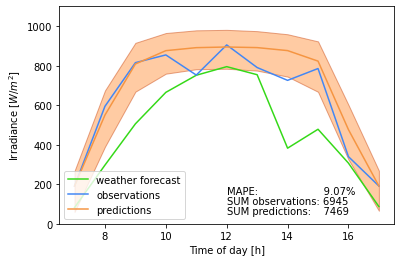
\includegraphics[scale=0.5]{imgs/graphs/full/medium/med_g_3.png}}\qquad
    \subfloat[Limited model]{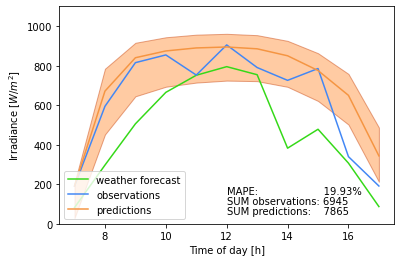
\includegraphics[scale=0.5]{imgs/graphs/less/medium/med_g_1.png}}\qquad
    \caption{Comparison of model performance on a day with some drops in irradiance.
    \label{fig:disc_med}}
\end{figure}

Fig.~\ref{fig:disc_high} shows a clear example of the performance difference between the models on erratic days. The full model, while still having a high error gets somewhat close to keeping the observations within its much smaller 90\% confidence interval than the limited model. The limited model also predicts much more irradiance over the day than the, already too high, full model.
\begin{figure}[ht!]
    \centering
    \subfloat[Full model]{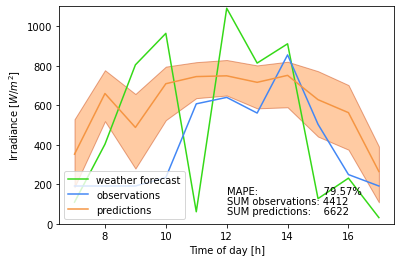
\includegraphics[scale=0.5]{imgs/graphs/full/high/high_3.png}}\qquad
    \subfloat[Limited model]{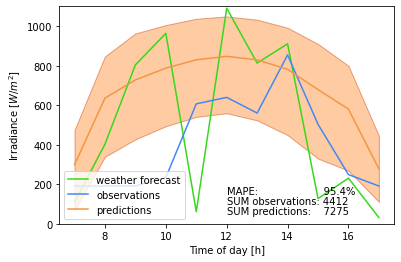
\includegraphics[scale=0.5]{imgs/graphs/less/high/high_4.png}}\qquad
    \caption{Comparison of model performance on an erratic day.
    \label{fig:disc_high}}
\end{figure}


\section{Conclusion\label{sec:conclusions}}
The results clearly show that relying forecast irradiance data from meteorological models is a very effective, but not perfect, method of accurately predicting irradiance in a single area. A transformer model, the Temporal Fusion Transformer, managed to very effectively translate patterns in meteorological irradiance forecasts to accurate local irradiance predictions utilizing spatially and temporally adjacent data.

We used a dataset of a fairly limited size, only 425 days. A few years of data for training the model would likely yield somewhat better results. The data can be processed more before being input into the network to account for known variables like daily and yearly swings in irradiance, which might improve performance. There exists satellite irradiance measurement data which might be used for improving accuracy. It would be interesting to see if a neural network could extract information from the seven pyranometers scattered across the power station, rather than only dropping the highest and lowest values and taking an average. 

Sadly, there is not a standard benchmark for solar irradiance forecast models, and the data used by others who have done similar work is not available, so we can't make a proper comparison between methodologies and models. 
%%% Local Variables: 
%%% mode: latex
%%% TeX-master: "DEGREE-NAME-YEAR"
%%% End: 
%%RUM: "Discussion"

%% ---------------------------------------------------------------
\printbibliography{} %%RUM: "References"

%% If appendices are needed, uncomment the following line
%% and include the appendices in separate files
\appendix{}%%RUM: "Appendicies (as appropriate)
\chapter{Code}\label{cha:code}
You can put code in your document using the listings package, which is
loaded by default in \path{custom.tex}.  Be aware that the listings
package does not put code in your document if you are in draft mode
unless you set the \texttt{forcegraphics} option.

There is an example java (Listing~\ref{src:Data_Bus.java}) and XML
file (Listing~\ref{src:AndroidManifest.xml}).  Thanks to the
\texttt{url} package, you can typeset OSX and unix paths like this:
\path{/afs/rnd.ru.is/project/thesis-template}.  Windows paths:
\path{C:\windows\temp\ }.  You can also typeset them using the menukey
package, but it tends to delete the last separator and has other
complications.\footnote{The menukey package has issues with biblatex,
  read \path{custom.tex} for more information.}

If you are trying to include multiple different languages, you should
go read the documentation and set these up in \path{custom.tex}.  You
will save yourself a lot of effort, especially if you have to fix
anything.

%I have put the source code in the \directory{src/} folder.
\lstinputlisting[language=Java, firstline=1,
lastline=40, caption={Data\_Bus.java: Setting up the class.},
label={src:Data_Bus.java}]{src/Data_Bus.java}

\lstinputlisting[language={[android]XML}, firstline=1, lastline=20,
caption={AndroidManifest.xml: Configuration for the Android UI.},
label={src:AndroidManifest.xml}]{src/AndroidManifest.xml}

%%% Local Variables: 
%%% mode: latex
%%% TeX-master: "DEGREE-NAME-YEAR"
%%% End: 
 % as an example, perhaps some of your code

%\backmatter{} % Sections after this don't get numbers
%% We prefer that all elements be numbered

%%%%%%%%%%%%% SHOW INDEX %%%%%%%%%%%%%%%%%%
%% Index, optional.  A good idea on longer documents

% You can put instructions at the beginning of the index:
%\renewcommand{\preindexhook}{%
%  The first page number is usually, but not always,
%  the primary reference to the indexed topic.\vskip\onelineskip}

%% You may have to run "makeindex <FILENAME>" to have it be generated
%% Depending upon which package you chose.
%% 
\clearforchapter{}
\printindex{}%%RUM: Not mentioned

%\backcover{}%%RUM: "Back cover (only Phd)
\end{document}

%% ---------------------------------------------------------------

%%% Local Variables:
%%% mode: latex
%%% TeX-master: t
%%% TeX-engine: xetex
%%% End:
